%!TEX root = ../template.tex
%%%%%%%%%%%%%%%%%%%%%%%%%%%%%%%%%%%%%%%%%%%%%%%%%%%%%%%%%%%%%%%%%%%%
%% chapter4.tex
%% NOVA thesis document file
%%
%% Chapter with lots of dummy text
%%%%%%%%%%%%%%%%%%%%%%%%%%%%%%%%%%%%%%%%%%%%%%%%%%%%%%%%%%%%%%%%%%%%

\typeout{NT FILE chapter4.tex}%

\chapter{Workplan}\label{cha:workplan}

In this chapter, we take a closer look at the workplan for the development and validation of the proposed solution.
To provide a clear overview of the workplan, we create a Gantt chart, displayed in Figure~\ref{fig:gantt}, and a table with the tasks and their respective description and tasks dependency. Our workplan is design for an estimated effort similar to the completed work for a Master Thesis, corresponding to 30 ECTS, meaning that we plan to spend 840 hours of work (30 ECTS * 28 hours/ECTS), for which we account for the possibility of a margin of error of 10\% in the total time. 

\section{Prototype Development}
To easily comprehend the impact of each module of our solution, both on privacy and performance, and to mitigate the risk of not being able to complete the work in the estimated time, we divided our solution into phases:

\subsection{Phase 1}
After revisioning the system model and the initial specification of the components, we will start by setting up the development environment and tools. This includes compiler and text editors installation, as well as some earlier testing, like launching a Tor node, to understand the system's behavior and provide evidence and useful knowledge for the development and testing of all prototypes. With everything set up and ready to go, we will start by extending the Tor Source Code and implement the \textit{Unobservability Scheduler} Prototype. Testing will also take place in this phase, as we will have to test the prototype, debug some possible code errors and evaluate its performance. At the end of this phase, it is expected that we will have a working prototype of the \textit{Unobservability Scheduler} on a Tor/MIRACE node, with Differential Private mechanisms and configurable parameters. At this point, we also aim to already have a set of tests that provide evidence of each parameter impact on the system's performance and privacy guarantees.

\subsection{Phase 2}

In this phase, we already have a working and tested prototype of the \textit{Unobservability Scheduler} on a Tor/MIRACE node. Now we need to enhance the client side of our system in order to maintain the privacy guarantees that we aim to provide, even in the presence of a fingerprinting attacker. We will build a Client Proxy capable of connecting to the Tor/MIRACE Network. By developing a proxy we intend to make the differential private mechanism on the client side and provide a seamless experience to the user. After developing the client proxy, we will test its basic functionalities. At the end of this phase, we assume that we have a working prototype of the \textit{Unobservability Scheduler} and a working prototype of the \textit{Client Proxy}, both with Differential Private mechanisms and configurable parameters.  

\subsection{Final Phase}
At last, we will merge both prototypes into a single solution, and perform a final validation and experimental evaluation. This phase is essential to provide clear evidence that our proposed solution is able to provide formal privacy guarantees to the users of the anonymization network. We expect some optimizations and validations to be necessary over both prototypes as we test them. At the end of this phase, we expect to have a final working prototype of a \textit{Differential Private Anonymization Network} that is able to provide formal privacy guarantees to its users, whilst maintaining practical levels of performance. We also intend to provide a set of observations and recommendations for the use of our system, related to used values of parameters, and the impact of the system's performance and privacy guarantees.


Upon completing these development phases, particular elements of the solution will be subject to thorough analysis and meticulous implementation:
\paragraph{Differential Privacy:} The main focus of this work is to provide a solution that is able to provide formal privacy guarantees to anonymization network's users. Formal privacy guarantees are an important aspect of our system, as it will provide a clear understanding of the privacy guarantees that users have when using our system. Therefore, we will have to implement the Differential Privacy mechanisms and evaluate its impact in the system's performance.
\paragraph{Flexible Configuration \& Parameterization:} Another important aspect of the work we want to develop is the ability to provide flexible behavior to the system. This flexibility can be divided into two main subjects: the users, and the correspondent needs and preferences, are one source of flexibility, and we consider important to provide a system that can be easily configured by the user and fit his needs. On the other hand, the system itself should be able to adapt to the real-time conditions that it is subject to. For example, the system should be able to adapt to the network's jitter and latency, and adapt the noise added to the messages accordingly, by modifying the privacy parameters. Therefore, our system will have a flexible configuration and parameterization, and a vast number of parameters lead to a vast range of tests that we will have to perform.  



\begin{figure}
    \centering
    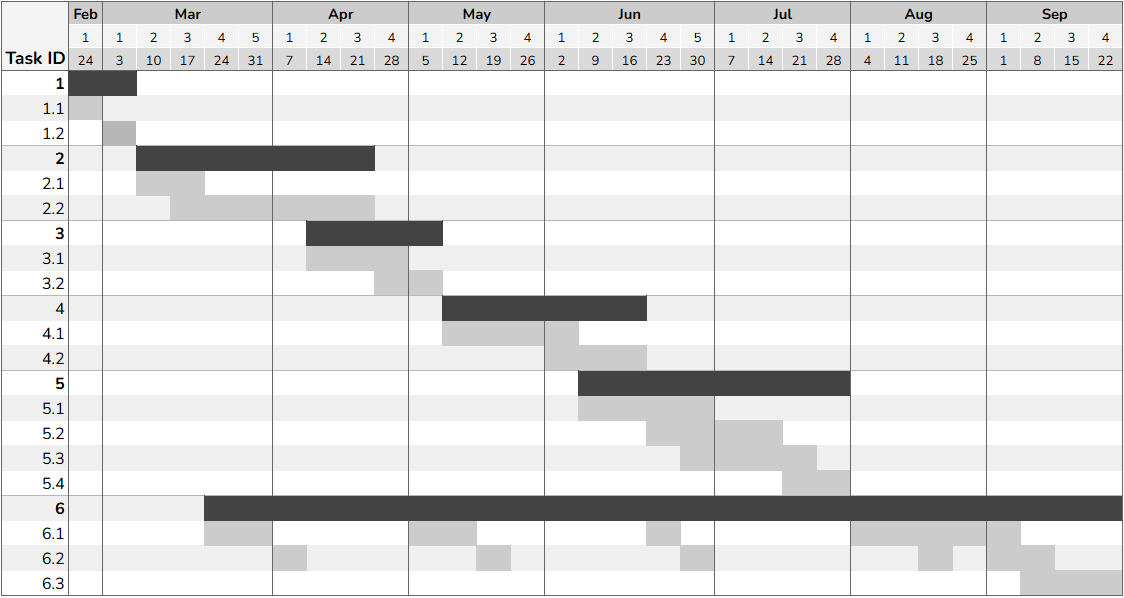
\includegraphics[width=\textwidth]{Chapters/Figures/Gantt.png}
    \caption{Gantt chart of the workplan}
    \label{fig:gantt}
\end{figure}

\section{Tasks \& Milestones}

In this section, we present a table with a more detailed overview of the tasks and their dependencies, as complement to the previously presented Gantt chart~\ref{fig:gantt}. The table is presented in Table~\ref{tab:table}.

\newcommand{\maintask}[3]{%
    \rowcolor[HTML]{E3E3E3} 
    \textbf{#1} & \textbf{#2} & \textbf{#3} & \textbf{} \\ \hline
}

\newcommand{\subtask}[4]{%
    #1 & #2 & #3 & #4 \\ \hline
}

\newcommand{\lastsubtask}[4]{%
    #1 & #2 & #3 & #4 \\ \hline
}

\begin{table}[h!]
    \centering
    \footnotesize
    \begin{tabular}{|c|p{5cm}|c|p{6cm}|}
        \hline
        \rowcolor[HTML]{C3C3C3} 
        \textbf{Task ID} & \textbf{Task} & \textbf{Dependency} & \textbf{Description} \\ \hline
        
        \maintask{1}{Revision \& Consolidation of Elaboration Guidelines}{}
        \subtask{1.1}{System Model \& Evaluation}{-}{Revision of the System Model}
        \subtask{1.2}{Initial Specification of Components}{1.1}{Consolidation of the Components Specification}

        \maintask{2}{Phase 1 Prototype}{}
        \subtask{2.1}{Setup Development Environment}{-}{Installation and Configuration of Development Environment \& Tools}
        \subtask{2.2}{Development}{2.1}{Development of Scheduler Prototype}

        \maintask{3}{Phase 1 Testing}{}
        \subtask{3.1}{Development of the first tests}{2.1}{Development of Test Environment and Tools}
        \subtask{3.2}{Testing}{3.1}{Testing of Scheduler Prototype}

        \maintask{4}{Phase 2 Prototype}{}
        \subtask{4.1}{Development}{3.2} {Development of Client Side Prototype}
        \subtask{4.2}{Testing}{4.1} {Testing of Client Side Prototype}

        \maintask{5}{Final Prototype}{}
        \subtask{5.1}{Consolidation}{4.1}{Consolidation of Phases 1 and 2 Prototypes}
        \subtask{5.2}{Validation \& Experimental Evaluation}{5.1}{Validation of Final Prototype}
        \subtask{5.3}{Optimizations \& Validations}{5.1}{Final Optimizations and Validations}
        \subtask{5.4}{Final Observations}{5.2, 5.3}{}

        \maintask{6}{Dissertation Report}{}
        \subtask{6.1}{Report Writing}{-}{}
        \subtask{6.2}{Report Revision}{-}{}
        \subtask{6.3}{Preparation for Presentation}{-}{}
    
    \end{tabular}
    \caption{Overview of tasks and their dependencies as presented in Figure~\ref{fig:gantt}}
    \label{tab:table}
\end{table}


